\documentclass[../main.tex]{subfiles}
\setlength{\columnsep}{4pt}
\begin{document}
\textit{The cool, refreshing water suddenly erupts in a storm of reaching, grasping tentacles. The tentacles connect to a primeval fish, 20 feet in length from its bulbous head to its crescent-shaped tail. Three slit-shaped eyes, protected by bony ridges, are set one atop the other in the front of its head, which remains just beneath the surface as it attacks.}

\noindent{The aboleth is a revolting fishlike amphibian found primarily in subterranean lakes and rivers. It despises all nonaquatic creatures and attempts to destroy them on sight.}\\
\indent{An aboleth has a pink belly. Four pulsating blue-black orifices line the bottom of its body and secrete grey slime that smells like rancid grease. It uses its tail for propulsion in the water and drags itself along with its tentacles on land. An aboleth weighs about 6,500 pounds.}\\
\indent{Aboleths are cruel and highly intelligent, making them dangerous predators. They know many ancient and terrible secrets, for they inherit their parent's knowledge at birth and assimilate the memories of all they consume.}\\
\indent{Aboleths are smart enough to refrain from immediately attacking land dwellers who draw near. Instead they hang back, hoping their prey will enter the water, which they often make appear cool, clear, and refreshing with their powers of illusion. Aboleths also use their psionic abilities to enslave individuals for use against their own companions.}\\
\indent{Aboleths have both male and female reproductive organs. They breed in solitude, laying 1d3 eggs every five years. These eggs grow for another five years before hatching into full-grown aboleths. Although the young are physically mature, they remain with their parent for some ten years, obeying the older creature utterly.}\\
\indent{Aboletsh speak their own language, as well as Undercommon and Aquan.}

\dndsection{COMBAT}
\noindent{An aboleth attacks by flailing with its long, slimy tentacles, though it prefers to fight from a distance using its illusion powers.}\\
\indent{\textbf{Enslave (Su):} Three times per day, an aboleth can attempt to enslave any living creature within 30 feet. The target must succeed on a DC 17 Will save or be affected as though by a \textit{dominate person} spell (caster level 16th). An enslaved creature obeys the aboleth's telepathic commands until freed by \textit{remove curse}, and can attempt a new Will save every 24 hours to break free. The control is broken if the aboleth dies or travels more than 1 mile from its slave. The save DC is Charisma-based.}\\
\indent{\textbf{Psionics (Sp):} At will--\textit{hypnotic pattern} (DC 15), \textit{illusory wall} (DC 17), \textit{mirage arcana} (DC 18), \textit{persistent image} (DC 18), \textit{programmed image} (DC 19), \textit{project image} (DC 20), \textit{veil} (DC 19). Effective caster level 16th. The save DCs are Charisma-based.}\\
\indent{\textbf{Slime (Ex):} A blow from an aboleth's tentacle can cause a terrible affliction. A creature hit by a tentacle must succeed on a DC 19 Fortitude save or begin transforming over the next 1d4+1 minutes, the skin gradually becoming a clear slimy membrane. An afflicted creature must remain moistened with cool fresh water or 1d12 points of damage every 10 minutes. The slime reduces the creature's natural armour bonus by 1 (but never to less than 0). The save DC is Constitution-based.}\\
\indent{A \textit{remove disease} spell cast before the transformation is complete will restore an afflicted creature to normal. Afterward, however, only a \textit{heal} or \textit{mass heal} spell can reverse the affliction.}\\
\indent{\textbf{Mucus Cloud (Ex):} An aboleth underwater surrounds itself with a vicious cloud of mucus roughly 1 foot thick. Any creature coming into contact with and inhaling this substance must succeed on a DC 19 Fortitude save or lose the ability to breath air for the next 3 hours. An affected creature suffocates in 2d6 minutes if removed from the water. Renewed contact with the mucus cloud and failing another Fortitude save continues the effect for another 3 hours. The save DC is Constitution-based.}\\
\indent{\textbf{Skills:} An aboleth has a +8 racial bonus on any Swim check to perform some special action or avoid hazard. It can always choose to take 10 on a Swim check, even if distracted or endangered. It can use the run action while swimming, provided it swims in a straight line.}

\dndsection{ABOLETH MAGE}
\noindent{Among the watery tombs and dungeons they inhabit, the lords of the aboleths focus their efforts to achieve dominion through their study of wizardry. Their great power marks them as among the lords of all subterranean creatures. Still, these creatures, devoted to their arcane scholarship, spend most of their long lives alone.}

\dndsubsection{Combat}
\noindent{The save DC for the aboleth mage's transformation tentacle attack (DC 21) and its mucus cloud (DC 21) are adjusted for its higher Constitution score. The save DC for its enslave ability (DC 16) is adjusted for its lower Charisma score, as are the save DCs dor its psionic ablities: \textit{Hypnotic pattern} (DC 14), \textit{illusory wall} (DC 16), \textit{mirage arcana} (DC 17), \textit{persistent image} (DC 17), \textit{programmed image} (DC 18), \textit{project image} (DC 19), \textit{veil} (DC 18). Effective caster level 16th.}\\
\indent{The aboleth mage uses a number of spells, such as \textit{displacement}, \textit{greater invisibility}, and \textit{wall of force}, to protect itself while seizing control of its foes with spells and innate abilities.}\\
\indent{\textit{Typical Wizard Spells Prepared} (4 / 6 / 5 / 4 / 4 / 3; save DC 15 + spell level): 0--\textit{daze}, \textit{detect magic} (2), \textit{resistance}; 1st--\textit{alarm}, \textit{charm person}, \textit{color spray}, \textit{mage armour}, \textit{magic missile} (2); 2nd--\textit{blur}, \textit{bull's strength}, \textit{darkness}, \textit{fox's cunning}, \textit{see invisibility}; 3rd--\textit{dispel magic}, \textit{displacement}, \textit{fly}, \textit{lightning bolt}; 4th--\textit{greater invisivbility}, \textit{phantasmal killer}, \textit{scrying}, \textit{stoneskin}; 5th--\textit{hold monster}, empowered \textit{lightning bolt}, \textit{wall of force}.}

% table

% Please add the following required packages to your document preamble:
% \usepackage[table,xcdraw]{xcolor}
% If you use beamer only pass "xcolor=table" option, i.e. \documentclass[xcolor=table]{beamer}
% \usepackage[normalem]{ulem}
% \useunder{\uline}{\ul}{}
\begin{table}[]
\centering
\begin{tabular}{p{9em}p{16em}p{20em}}
 & \textbf{Aboleth} & \textbf{Aboleth Mage, 10th-Level Wizard} \\
 & \textbf{Huge Aberration (Aquatic)} & \textbf{Huge Aberration (Aquatic)} \\
\rowcolor[HTML]{FFCE93}
\textbf{Hit Dice:} & 8d8 + 40 (76 hp) & 8d8 + 56 plus 10d4 + 70 (177 hp) \\
\textbf{Initiative:} & +1 & +7 \\
\rowcolor[HTML]{FFCE93}
\textbf{Speed:} & 10 ft. (2 squares), swim 60 ft. & 10 ft. (2 squares), Swim 60 ft. \\
\textbf{Armor Class:} & 16 (-2 size, +1 Dex, +7 natural), touch 9, flat-footed 15 & 18 (-2 size, +3 Dex, +7 natural), touch 11, flat-footed 15 \\
\rowcolor[HTML]{FFCE93}
\textbf{Base Attack/Grapple:} & +6/+22 & +11/+28 \\
\textbf{Attack:} & Tentacle +12 melee (1d6+8 plus slime) & Tentacle +18 melee (1d6+9 plus slime) \\
\rowcolor[HTML]{FFCE93}
\textbf{Full Attack:} & 4 tentacles +12 melee (1d6+8 plus slime) & 4 tentacles +18 melee (1d6+9 plus slime) \\
\textbf{Space/Reach:} & 15 ft./10 ft. & 15 ft./10 ft. \\
\rowcolor[HTML]{FFCE93}
\textbf{Special Attacks:} & Enslave, psionics, slime & Enslave, psionics, slime \\
\textbf{Special Qualities} & Aquatic subtype, darkvision 60 ft., mucus cloud & Aquatic subtype, darkvision 60 ft., mucus cloud, summon familiar \\
\rowcolor[HTML]{FFCE93}
\textbf{Saves:} & Fort +7, Ref +3, Will +11 & Fort +15, Ref +10, Will +15 \\
\textbf{Abilities:} & Str 26, Dex 12, Con 20, Int 15, Wis 17, Cha 17 & Str 28, Dex 16, Con 24, Int 20, Wis 16, Cha 14 \\
\rowcolor[HTML]{FFCE93}
\textbf{Skills:} & Concentration +16, Knowledge (any one) +13, Listen +16, Spot +16, Swim +8 & Bluff +13, Concentration +25, Decipher Script +15, Diplomacy +6, Disguise +2 (+4 acting), Intimidate +4, Knoledge (arcana) +15, Knowledge (dungeoneering) +25, Knowledge (history) +15, Knowledge (the planes) +15, Listen +15, Search +10, Sense Motive +15, Spellcraft +20, Spot +17, Survival +3 (+5 following tracks, on other planes, and underground), Swim +8 \\
\textbf{Feats:} & Alertness, Combat Casting, Iron Will & Combat Casting, Empower Spell, Eschew Materials, Great Fortitude, Improved Initiative, Lightning Reflexes, Scribe Scroll, Spell Focus (illusion), Spell Focus (enchantment), Spell Penetration \\
\rowcolor[HTML]{FFCE93}
\textbf{Environment:} & Underground & Underground \\
\textbf{Organisation:} & Solitary, brood (2-4), or slaver brood (1d3+1 plus 7-12 skum) & Solitary \\
\rowcolor[HTML]{FFCE93}
\textbf{Challenge Rating:} & 7 & 17 \\
\textbf{Treasure:} & Double standard & Double standard \\
\rowcolor[HTML]{FFCE93}
\textbf{Alignment:} & Usually lawful evil & Usually lawful evil \\
\textbf{Advancement:} & 9-16 HD (Huge); 17-24 HD (Gargantuan) & By character class \\
\rowcolor[HTML]{FFCE93}
\textbf{Level Adjustment:} & --- & ---
\end{tabular}
\end{table}

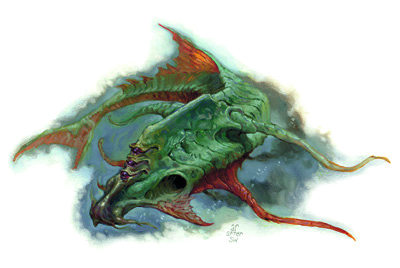
\includegraphics[width=\columnwidth]{Aboleth}

\end{document}
